\documentclass[12pt]{article}

%Packages add more power to LaTeX documents
\usepackage{fullpage} %Otherwise there will be a lot of wasted space at the margins
\usepackage{enumerate} %For the multi-part problem in example #4
\usepackage{amsthm} %For proof environment
\usepackage{amsmath} %For math symbols (like the black square)
\usepackage{graphicx,float,wrapfig} %Including graphics like PDFs and some image formats.


\author{Annabelle Cormia}
\title{CSCI 430: Homework 1}


\begin{document}
\maketitle

Tyler Archer, Paul Gosser, Robert Rayburn, and I collaborated on this assignment.\newline

\section{Chapter 1.1 (1.1-1 through 1.1-5)}

%Number \item tags
\begin{enumerate}
 
  \item Cataloguing and shelving library books is a real-world example that requires sorting.

  \item Efficiency may be measured in resources needed to accomplish a certain task. An efficient method would use less resources than a less efficient method.
    
  \item Strengths of a Queue: First-In First-Out (FIFO), so queues are useful for storing things in chronological order. It is very simple to access the first and last element of a queue. \newline \newline Limitations of a Queue: Access is not constant, so searching in a queue is O(N).

  \item The problems are similar in that they are both trying to find the minimum distance traveled. However, they are different in that the traveling-salesman problem must hit every point and then end up at the same point it started at, while the shortest-path problem just finds the shortest path between two different points and it is not required to visit every point.

  \item One example of a real-world problem when only the best will do would be a flight where the traveler has meetings scheduled at 9:00 and 2:00 in different locations (assuming the same time zone). The traveler must leave at 10:00 and arrive at her destination two hours before her next meeting at 2:00. Therefore, only the best flight time with the most efficient path will be acceptable in order to allow her to attend her meeting. \newline \newline An example where "approximately" the best is good enough would be when climbing a mountain. Someone climbing a mountain may not choose the most best and most efficient path to the top, but they will still get to the top.
    
\end{enumerate}

\section{Chapter 1.2 (1.2-1 through 1.2-3)}

%Number \item tags
\begin{enumerate}
    
  \item An example of an application that requires algorithmic content at the application level would be Facebook. Facebook requires a search algorithm to allow the user to search for friends and pages. Another example would be the sorting algorithm that Facebook uses to push the "most interesting" stories to the top of the user's feed.
    
  \item Assuming lg is base 2, insertion sort beats merge for for approximate values $1 \leq n \leq 43$. \newline $64nlg(n) \geq 8n^2$ \newline $8nlg(n) \geq n^2$ \newline $8lg(n) \geq n$ \newline $8lg(n)-n \geq 0$ \newline I then used Wolram Alpha as a calculator to graph the problem, and I found the range between approximately 1 and 43 to be the solution. See Figure \ref{figure1}. \newline 

\begin{figure}[h!]
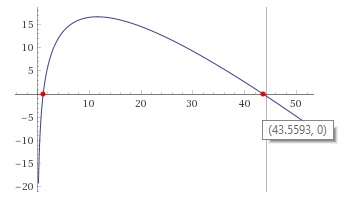
\includegraphics[width=7cm]{Graph.jpg}
\centering
\caption{Wolfram Alpha calculation.}
\label{figure1}
\end{figure}
    
  \item The smallest value of n such that an algorithm whose running time is $100n^2$ runs faster than an algorithm whose running time is $2^n$ on the same machine is approximately n=15. See Figure \ref{figure2}. \newline 

\begin{figure}[h!]
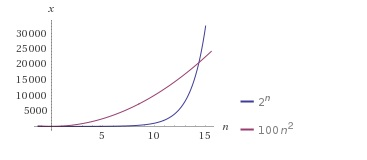
\includegraphics[width=9cm]{Graph2.jpg}
\centering
\caption{Wolfram Alpha calculation.}
\label{figure2}
\end{figure}
    
\end{enumerate}
    
\end{document}